
%(BEGIN_QUESTION)
% Copyright 2008, Tony R. Kuphaldt, released under the Creative Commons Attribution License (v 1.0)
% This means you may do almost anything with this work of mine, so long as you give me proper credit

A technician is troubleshooting a power supply circuit that outputs substantially less DC voltage than it should.  The output voltage is supposed to be 15 volts DC under load, but instead it is actually outputting less than 8 volts DC under load:

$$\includegraphics[width=15.5cm]{i03177x01.eps}$$

The technician measures approximately 12 volts AC (RMS) across the secondary winding of the transformer.  Based on this voltage measurement and the knowledge that there is reduced DC output voltage, identify two possible faults (either one of which could account for the problem and all measured values in this circuit), and also identify two circuit elements that could not possibly be to blame (i.e. two things that you know {\it must} be functioning properly, no matter what else may be faulted).  The circuit elements you identify as either possibly faulted or properly functioning can be wires, traces, and connections as well as components.  Be as specific as you can in your answers, identifying both the circuit element and the type of fault.

\medskip
\goodbreak
\item{} Circuit elements that are possibly faulted
\item{1.} 
\item{2.} 
\end{itemize}

\medskip
\goodbreak
\item{} Circuit elements that must be functioning properly
\item{1.} 
\item{2.} 
\end{itemize}

\vfil 

\underbar{file i03177}
\eject
%(END_QUESTION)





%(BEGIN_ANSWER)

This is a graded question -- no answers or hints given!

%(END_ANSWER)





%(BEGIN_NOTES)

We know we're getting at least {\it some} DC voltage out of this power supply, so the fault cannot be anything that would kill all the output (e.g. blown fuse, failed-open transformer winding, etc.).  The AC voltage measurement at the transformer's secondary winding confirms this.

The only faults which could cause a partial DC output voltage despite full AC voltage coming from the transformer's secondary winding are limited to the bridge rectifier subcircuit.  Any one of these diodes failing open could account for what we're seeing.

\medskip
\goodbreak
\item{} Circuit elements that are possibly faulted
\item{1.} Diode D1 (open)
\item{2.} Diode D2 (open)
\item{3.} Diode D3 (open)
\item{4.} Diode D4 (open)
\end{itemize}

\medskip
\goodbreak
\item{} Circuit elements that must be functioning properly
\item{1.} AC power source (wall receptacle)
\item{2.} Fuse
\item{3.} All PCB traces on the line-voltage side
\item{4.} Transformer
\end{itemize}

%INDEX% Troubleshooting review: electric circuits

%(END_NOTES)


